\documentclass[10pt, letterpaper]{article}
\usepackage[letterpaper, top=2.2cm, bottom=2.4cm, left=2.3cm, right=2.3cm]{geometry}
\usepackage[T1]{fontenc}
\usepackage{amsmath, amssymb}
\usepackage{newtxtext}
\usepackage[scaled=0.92]{helvet}
\let\Bbbk\relax
\usepackage{newtxmath}
\usepackage{graphicx}
\usepackage{titlesec}
\usepackage{xcolor}
\usepackage{caption}
\usepackage{fancyhdr}
\usepackage[hidelinks]{hyperref}

\definecolor{sec}{RGB}{22,45,74}
\titleformat{\section}{\sffamily\large\bfseries\color{sec}}{\thesection}{0.6em}{}
\captionsetup{labelfont={bf,sf}, font=small, labelsep=period}
\renewcommand{\thefigure}{S\arabic{figure}}
\renewcommand{\thetable}{S\arabic{table}}
\pagestyle{fancy}\fancyhf{}
\renewcommand{\headrulewidth}{0pt}
\fancyhead[L]{\sffamily\footnotesize\color{sec}Supplementary Information}
\fancyfoot[C]{\sffamily\footnotesize S\thepage}

\title{\sffamily\bfseries\color{sec}Supplementary Information\\[2pt]
\large\mdseries Symmetry, not information, determines what a predictive cognitive map collapses}
\author{\sffamily Manas Venkata Sai Ravulapalli}
\date{}

\begin{document}
\maketitle

\noindent This document collects supporting figures for the main text. All panels are generated
directly from the result files by \texttt{project5\_symmetry/analysis/make\_paper\_figures.py} and
\texttt{rate\_maps.py}; no values are entered by hand.

\section{Place-field rate maps, all extracted units}

The main-text place-cell figure shows a small number of example units per condition. To show that
this selection is representative rather than chosen, the following figures give the full set of
extracted units for each condition, ranked by Skaggs spatial information and left otherwise
unselected. Each tile is one unit's mean firing-rate map over the arena, smoothed for display and
normalised to its own peak.

\begin{figure}[h!]
\centering
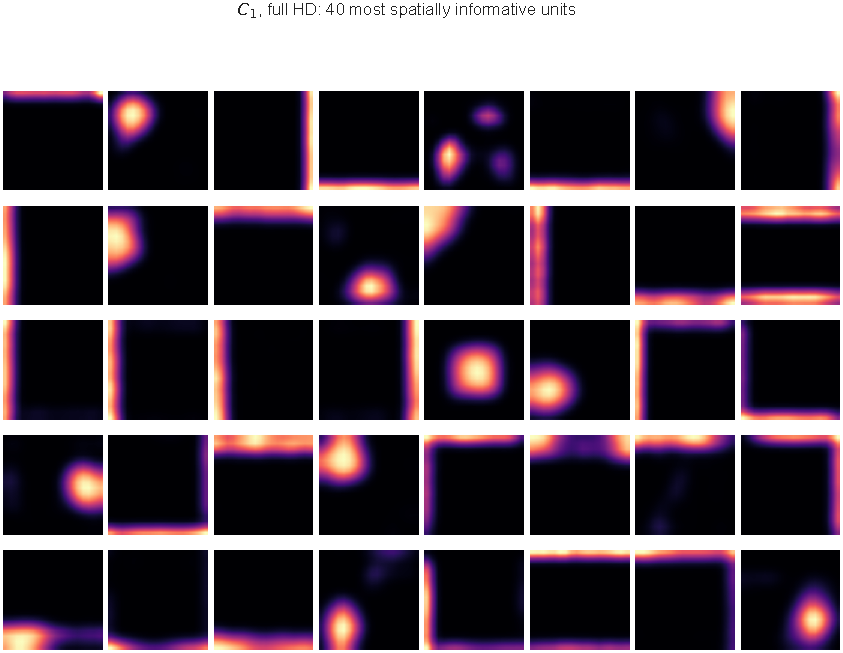
\includegraphics[width=\textwidth]{figures/figS_units_s1_full.pdf}
\caption{Asymmetric arena, full head-direction encoding. Units carry single, sharp place fields.}
\end{figure}

\begin{figure}[h!]
\centering
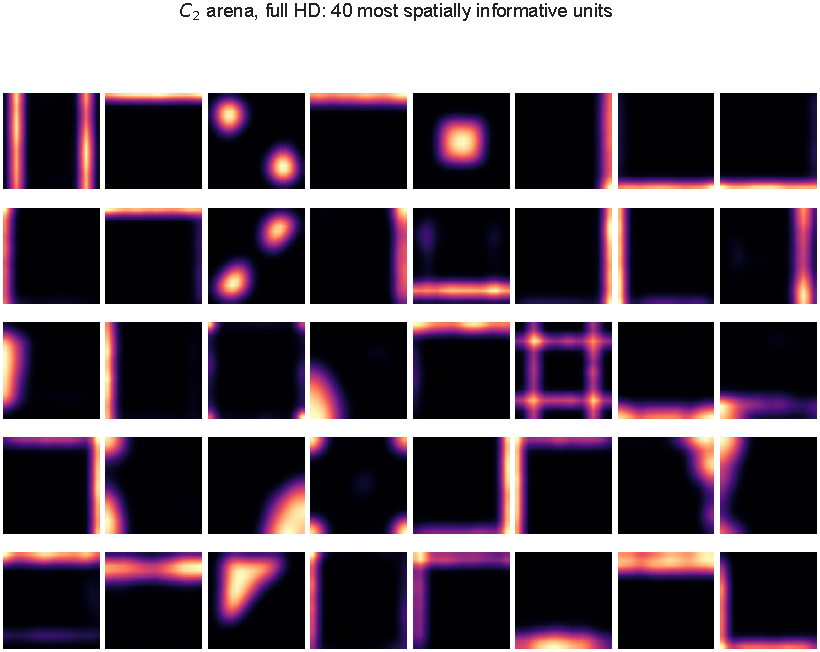
\includegraphics[width=\textwidth]{figures/figS_units_s2_full.pdf}
\caption{$C_2$ arena, full head-direction encoding. With the full compass available the fields do
not systematically repeat.}
\end{figure}

\begin{figure}[h!]
\centering
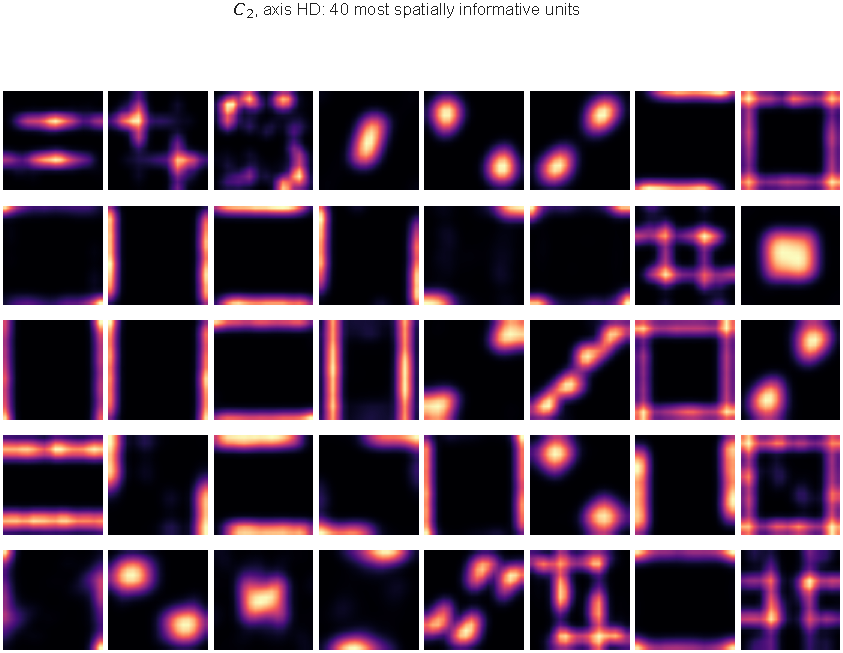
\includegraphics[width=\textwidth]{figures/figS_units_s2_axis.pdf}
\caption{$C_2$ arena, \textit{axis} encoding. The encoding is invariant under the $180^\circ$
rotation, and fields repeat at $180^\circ$-related locations across the population.}
\end{figure}

\begin{figure}[h!]
\centering
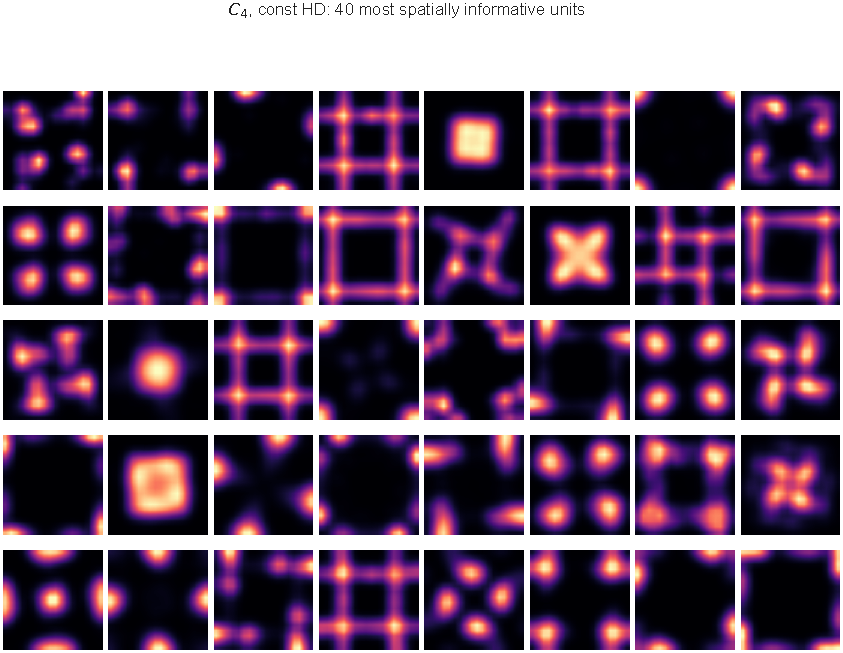
\includegraphics[width=\textwidth]{figures/figS_units_s4_const.pdf}
\caption{$C_4$ arena, \textit{const} encoding. The encoding is invariant under the full $C_4$
group, and fields repeat at all four $90^\circ$-related locations.}
\end{figure}

\clearpage
\section{Population manifolds of the topology arenas}

\begin{figure}[h!]
\centering
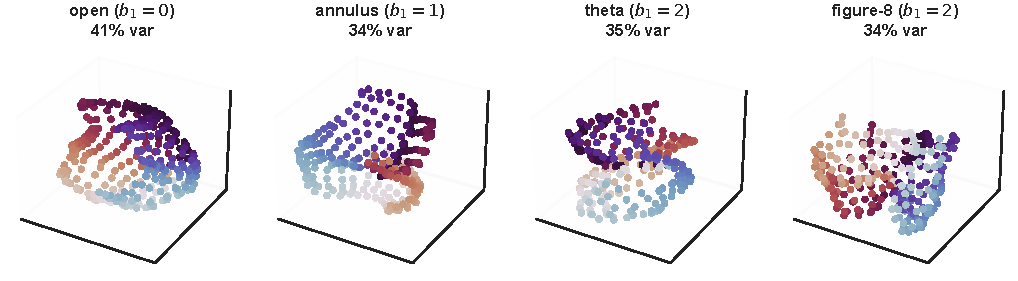
\includegraphics[width=\textwidth]{figures/fig_manifold_pc.pdf}
\caption{Position-conditioned population manifolds for the four topology arenas, PCA to three
dimensions (one point per passable cell, coloured by angle around the arena centre). Position is
mapped smoothly in every arena, but the manifolds are high-dimensional: three principal
components capture only $34$--$41\%$ of the variance, and no low-dimensional loop is visible even
for the annulus ($b_1 = 1$) or the theta and figure-8 arenas ($b_1 = 2$). This is consistent
with the persistent-homology analysis, which does not recover the arenas' loop topology (main
text, Limitations): the code is metrically organised well before, and without ever cleanly
acquiring, the arena's topology.}
\end{figure}

\clearpage
\section{Map quality and offline replay}

\begin{figure}[h!]
\centering
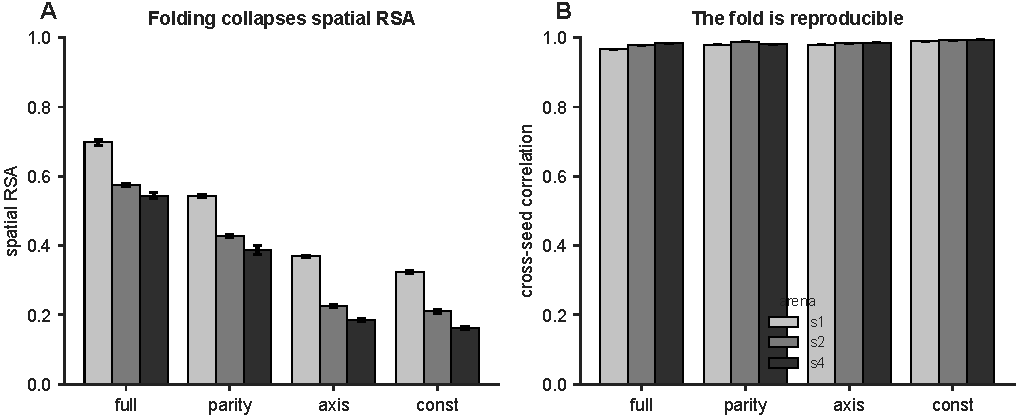
\includegraphics[width=\textwidth]{figures/fig_map_quality.pdf}
\caption{Spatial representational similarity falls as the head-direction encoding is ablated and as
arena symmetry increases (left), while the cross-seed correlation between independently trained
networks stays high (right). A folded code is reproducible rather than degenerate.}
\end{figure}

\begin{figure}[h!]
\centering
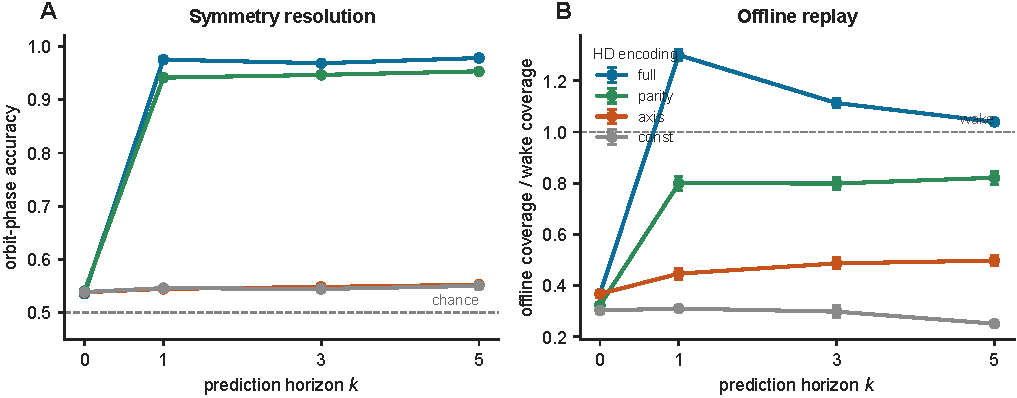
\includegraphics[width=\textwidth]{figures/fig_horizon.pdf}
\caption{Symmetry resolution (left) and offline replay coverage (right) as a function of the
prediction horizon $k$, for the four head-direction encodings in the $C_2$ arena. Both step up at
$k=1$ and are graded by how much of the compass the encoding retains.}
\end{figure}

\begin{figure}[h!]
\centering
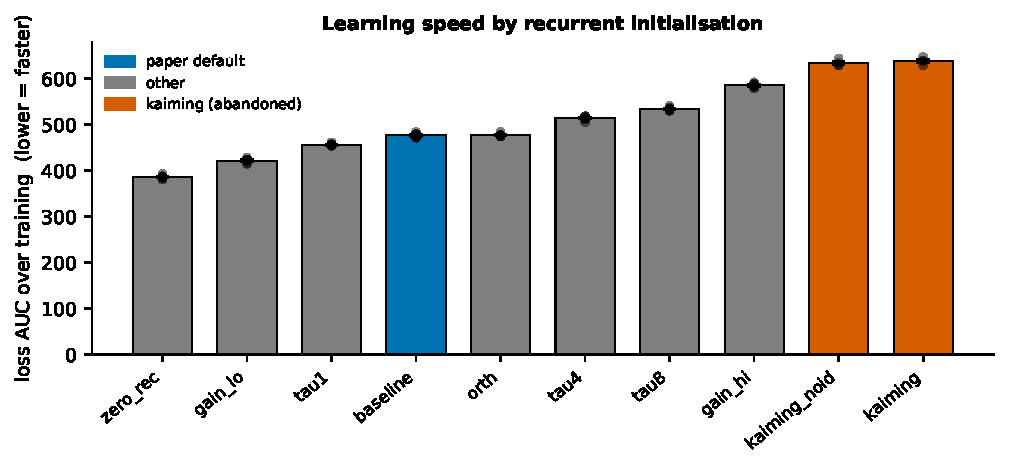
\includegraphics[width=0.7\textwidth]{figures/fig_init.pdf}
\caption{Learning speed by recurrent initialisation, measured as area under the training-loss curve
(lower is faster). A pure leak learns fastest; the abandoned Kaiming initialisation is slowest but
converges without instability.}
\end{figure}

\end{document}
